\documentclass{beamer}
\usetheme{metropolis}
\usepackage{xcolor}
\usepackage{graphicx}


% Supabase color palette
\definecolor{supabasegreen}{HTML}{3ECF8E}
\definecolor{supabasedark}{HTML}{1F1F1F}

% Dark theme settings
\setbeamercolor{background canvas}{bg=supabasedark}
\setbeamercolor{normal text}{fg=white,bg=supabasedark}
\setbeamercolor{frametitle}{fg=white,bg=supabasegreen}
\setbeamercolor{progress bar}{fg=supabasegreen}
\setbeamercolor{title}{fg=supabasegreen}
\setbeamercolor{structure}{fg=supabasegreen}

\usepackage{graphicx}
\usepackage{booktabs}
\usepackage{hyperref}

\title{Menu Generation Assistant}
\subtitle{Flutter + Supabase App}
\author{Haotian Sun, Dominic Pöltl, Joshua Lympany \\ \textbf{University of Tübingen}} 
\date{23.05.2025}
\institute{Department of Marketing}

\begin{document}

\begin{frame}
    \titlepage
\end{frame}

\begin{frame}{Outline}
    \tableofcontents
\end{frame}




\section{Application and User Stories}
\begin{frame}{User Story Examples (1)}
  \begin{itemize}
    \item \textbf{Image Upload}  
      \begin{itemize}
        \indent As a user, I want to upload a photo of my ingredients so that I can get a recipe suggestion.
      \end{itemize}
                  \vspace{2mm}
    \item \textbf{Preferences}  
      \begin{itemize}
        \indent As a user, I want to tell the App that I am vegan, or that I am looking to lose fat.
      \end{itemize}
  \end{itemize}
\end{frame}

\begin{frame}{User Story Examples (2)}
  \begin{itemize}
    \item \textbf{Ingredient Edit}  
      \begin{itemize}
        \indent As a user, I want to adjust detected ingredients so that the recipe matches my pantry. (even AI can make mistakes)
                    \vspace{2mm}
      \end{itemize}
    \item \textbf{Recipe Share}  
      \begin{itemize}
        \indent As a user, I want to share my generated recipe via link so that friends can view it.
      \end{itemize}
  \end{itemize}
\end{frame}


\begin{frame}{Potential Applications}
  \begin{itemize}
    \item \textbf{Smart Cooking Guide}  
      \begin{itemize}
        \indent Personalized step-by-step instructions based on ingredients
      \end{itemize}
      \vspace{1mm}
    \item \textbf{Quick Cooking Advisor}  
      \begin{itemize}
        \indent Instant recipe suggestions for meals under 15 minutes
      \end{itemize}
            \vspace{1mm}
    \item \textbf{Meal Planning \& Tracking}  
      \begin{itemize}
        \indent Auto-generate weekly menus and calorie logs from photos
      \end{itemize}
            \vspace{1mm}
    \item \textbf{Minimalist Recipe Generator}  
      \begin{itemize}
        \indent Create tasty dishes using only 3–5 ingredients on hand
      \end{itemize}
  \end{itemize}
\end{frame}



\section{Reasoning}
\begin{frame}{Core Principles}
  \begin{center}
    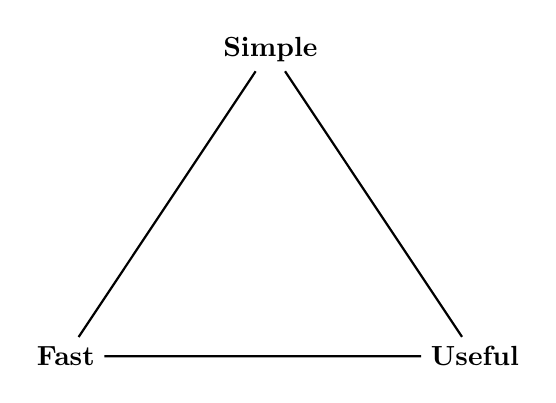
\begin{tikzpicture}[scale=2]
    
      % vertices
      \node (A) at (90:1.2cm)  {\textbf{Simple}};
      \node (B) at (210:1.5cm) {\textbf{Fast}};
      \node (C) at (-30:1.5cm) {\textbf{Useful}};
      % draw all three edges
      \draw[thick] (A) -- (B) -- (C) -- cycle;
      \draw[thick] (C) -- (A);
    \end{tikzpicture}
  \end{center}
\end{frame}
% ------------------ FRONT END ------------------
\section{Front End}


\begin{frame}{App Purpose}
    \begin{block}{\textbf{Image-to-Recipe Flutter App  
\includegraphics[width=0.05\textwidth]{pic1.png}}}
        \begin{itemize}
            \item Turns a food image into a custom recipe using AI
            \item Full pipeline: \\   \hspace{5mm} Upload → Extract → Generate → Display
            \item Built using Flutter with multi-screen navigation
            \item Emphasis on intuitive UX and fast processing
        \end{itemize}
    \end{block}
\end{frame}

\begin{frame}{User Flow}
    \begin{block}{\textbf{4-Stage Pipeline}}
        \begin{itemize}
            \item \textbf{Upload}: User selects a food image \textit{+ optional preferences}
            \item \textbf{Extract}: Ingredients extracted \textit{+ user adjustments} 
            \item \textbf{Generate}: Recipe created using ingredients
            \item \textbf{Display}: Recipe shown in structured format
        \end{itemize}
    \end{block}
\end{frame}

\begin{frame}{Page Structure}
    \begin{block}{\textbf{Modular Screen Architecture}}
        \begin{itemize}
            \item Each step implemented as a separate Flutter page
            \item Navigation via named routes
            \item Clear state transfer across stages
            \item Encourages scalability and decoupled logic
        \end{itemize}
    \end{block}
\end{frame}





% ------------------ BACK END ------------------
\section{Back End}

\begin{frame}{Back-End Overview}
    \begin{block}{\textbf{Cloud-Driven Actions by Supabase 
\includegraphics[width=0.05\textwidth]{pic2.jpeg}}}
        \begin{itemize}
            \item Handles image storage, user data, and AI inference
            \item Combines Supabase (database/storage/auth) with Google AI (vision + language)
            \item All processing offloaded to cloud for scalability
        \end{itemize}
    \end{block}
\end{frame}

\begin{frame}{Supabase Services}
    \begin{itemize}
        \item \textbf{Storage}: Uploaded food images stored securely
        \item \textbf{Database}: Stores user history, ingredients, recipes
        \item \textbf{Authentication}: Optional login support for personalization
        \item Fast RESTful API interface via Supabase SDK
    \end{itemize}
\end{frame}

\begin{frame}{Google AI APIs}
    \begin{itemize}
        \item \textbf{Vision AI}: Extracts ingredient keywords from image
        \item \textbf{Gemini API}: Generates recipe html from ingredients/preferences
        \item 2-shot API calls for each user story
        \item Reliable and scalable with minimal backend setup
    \end{itemize}
\end{frame}

\begin{frame}{Security \& Scalability}
    \begin{itemize}
        \item Supabase Row-Level Security for user-specific data
        \item Image access is signed and time-limited
        \item Backend logic can scale with serverless functions
        \item Easy to add monitoring or logging via Supabase or Google Cloud
    \end{itemize}
\end{frame}






\end{document}